\documentclass[linenumbers,RNAAS,trackchanges]{aastex631}
\usepackage[utf8]{inputenc}
\usepackage{hyperref}           % hrefs
\usepackage{natbib}             % for bibliography
\usepackage{float}              % figure positioning
\usepackage{svg}                % used for SVG images
\usepackage{graphicx}           % used for non-SVG images
\usepackage{csvsimple}
% Search Query Metadata
\shorttitle{Chaos in the Double Pendulum}
\shortauthors{Ajaykumar, et al.}

% Hyperlink setup
\hypersetup{
colorlinks=true,
linkcolor=blue,
urlcolor=blue
}

\begin{document}
\title{Investigating the Chaotic Nature of the Double Pendulum System}
% [] is for ORCiD
\correspondingauthor{}
\email{nikhitaajaykumar@utexas.edu, khernandez@utexas.edu, darryl.tran@utexas.edu}
\author{Nikhita Ajaykumar}

\author{Kayla Hernandez}

% or 
% \nocollaboration{0}

\author{Darryl Tran}
\affiliation{University of Texas at Austin\\
110 Inner Campus Drive\\
Austin, TX 78705}

% 250 word limit for abstract
\begin{abstract}
When studying the problem of the ideal single pendulum, there are a limited amount of factors that affect its movement. Such factors include gravity, the length of the string, the mass of the pendulum, and air resistance. However, attaching a second pendulum to the first pendulum produces movements that are chaotic. This experiment is known as the double pendulum. The equations derived to model the movements of the pendulums seem nearly impossible to solve analytically, calling for a numerical solution. This paper will explore the movements of the pendulums using a robust numerical method, the Runge-Kutta method. 
\end{abstract}

% Use astrothesaurus numbers in place of num
\keywords{Runge-Kutta (1) --- Double pendulum (2) --- Chaos (3)}
\section{Introduction} \label{sec:intro}
	The double pendulum is comprised of two pendulums. The pivot of the second pendulum is located at the end of the first pendulum, with both pendulums restrained to oscillating on the same plane.  
 
	Euler and Bernoulli first studied the complex dynamics of the double pendulum system in the 1730s. Both Euler and Bernoulli studied varying oscillations and how the double pendulum problem can be generalized to an n-pendulum problem. \cite{acheson_1998} Bernoulli found that for small motions, the double pendulum displayed both a low and high frequency of oscillation, displaying a chaotic behavior \cite{acheson_1998}. The double pendulum system contributed to the emerging Chaos Theory stemming from classical mechanics problems. Euler and Bernoulli understood that the solution to the double pendulum problem, much like many problems of motion during this period of attempting to solve and further understand classical mechanics, could be solved through differential equations. However, it was not until the recent advent of computers that the double pendulum could be further studied given that the solutions to the differential equations could only be solved numerically. 
 
	The manner in which the double pendulum manifests non-linear behavior not only gave rise to many theoretical contributions to the field of mechanics but also led to many practical applications. The double pendulum is also widely used in several modeling applications including robotics and human locomotion analysis.\cite{low}
 
	In this paper, we will be analyzing the simple double pendulum problem using the Runge-Kutta method in order to investigate the quasi-harmonic and chaotic motion of the double pendulum system. 


 
\
\section{Problem to be Solved} \label{sec:problem}
The motion of a double pendulum will be investigated using the Runge-Kutta method. The rods connected to the bobs will be considered massless, and air resistance will not be considered. Using geometry, the equations for the position of the pendulum are:


\begin{center}
\begin{tabular}{ l l }
 $x_1 = L_1 \sin(\theta_1)$ & $y_1 = -L_1 \cos(\theta_1)$  \\ 
 $x_2 = x_1 + L_2 \sin(\theta_2)$ & $y_2 = y_1 - L_2 \cos(\theta_2)$    
\end{tabular}
\end{center}

By differentiating, the equations for velocity are:

\begin{center}
\begin{tabular}{ l l }
 $\dot x_1 = \dot\theta_1 L_1 \cos(\theta_1)$ & $\dot y_1 = \dot\theta_1 L_1 \sin(\theta_1)$  \\ 
 $\dot x_2 = \dot x_1 + \dot\theta_2 L_2 \cos(\theta_2)$ & $\dot y_2 = \dot y_1 + \dot\theta_2 L_2 \sin(\theta_2)$    
\end{tabular}
\end{center}

Differentiating again, the equations for acceleration are:

\begin{center}
\begin{tabular}{ l l }
 $\ddot x_1 = -\dot\theta_1^2 L_1 \sin(\theta_1) + L_1 \cos(\theta_1) \ddot\theta_1$ & $\ddot y_1 = \dot\theta_1^2 L_1 \cos(\theta_1) + L_1 \sin(\theta_1) \ddot\theta_1$  \\ 
 $\ddot x_2 = \ddot x_1 - \dot\theta_2^2 L_2 \sin(\theta_2) + \ddot\theta_2 L_2 \cos(\theta_2)$ & $\ddot y_2 = \ddot y_1 + \dot\theta_2^2 L_2 \cos(\theta_2) + \ddot\theta_2 L_2 \sin(\theta_2)$    
\end{tabular}
\end{center}


\section{Differential equations} \label{sec:method}

Considering the forces acting on the double pendulum, more equations can be derived:


$$\sin(\theta_1) (m_1\ddot y_1 + m_2 \ddot y_2 + m_1 g + m_2 g) = -\cos(\theta_1)(m_1 \ddot x_1 + m_2 \ddot x_2)$$ 

and 

$$\sin(\theta_2) (m_2 \ddot y_2 + m_2 g) = -\cos(\theta_2) (m_2 \ddot x_2)$$

The equations where $\ddot\theta_1$ and $\ddot\theta_2$ are isolated were taken from a website by Erik Neumann \cite{neumann}. Since these are two 2nd order differential equations, the variable $\omega$ will be substituted for $\dot\theta$ and $\dot\omega$ for $\ddot\theta$. This is done to achieve four first order differential equations:

$$\dot\theta_1 = \omega_1$$

$$\dot\omega_1 = \frac{-g (2m_1 + m_2) \sin(\theta_1) - m_2 g \sin(\theta_1 - 2\theta_2) - 2\sin(\theta_1 - \theta_2) m_2 (\omega_2^2 L_2 + \omega_1^2 L_1 \cos(\theta_1 - \theta_2))}{L_1 (2m_1 + m_2 - m_2 \cos(2\theta_1 - 2\theta_2))}$$

$$\dot\theta_2 = \omega_2$$

$$\dot\omega_2 = \frac{2\sin(\theta_1 - \theta_2)(\omega_1^2 L_1 (m_1 + m_2) + g(m_1 + m_2) \cos(\theta_1) + \omega_2^2 L_2 m_2 \cos(\theta_1 - \theta_2))}{L_1 (2m_1 + m_2 - m_2 \cos(2\theta_1 - 2\theta_2))}$$


These equations will be solved using the Runge-Kutta method. The equations used for the Runge-Kutta method are as follows:

$$\frac{dx}{dt} = f(x,t), x(t_0) = x_0$$

$$k_1 = f(t_n, x_n)$$

$$k_2 = f(t_n + \frac{h}{2}, x_n + \frac{h}{2}k_1)$$

$$k_3 = f(t_n + \frac{h}{2}, x_n + \frac{h}{2}k_2)$$

$$k_4 = f(t_n + h, x_n + h k_5)$$

$$x_{(n+1)} = x_n + \frac{h}{6}(k_1 + 2k_2 + 2k_3 + k_4)$$

Where 

$$\frac{d\theta}{dt} = \omega$$

and

$$\frac{d\omega}{dt} = -\mu\omega - \frac{g}{L}\sin(\theta)$$

\section{Results} \label{sec:results}
While running the experiments, there are 4 parameters that is being varied. The ratio of the lengths of the two strings, the ratio of the two masses, the initial angle of the pendulums, and the initial angles of the masses. The experiment was run for 50 seconds with initial conditions. The length of the 2 strings ($L_{1}$, $L_2$) and the two masses ($m_1$, $m_2$) were set to equal each other at 1.0 meters and 0.1 kilograms respectively. The initial angles ($\theta_1$, $\theta_2$) were set to $\pi/30$ in radians and the initial angular velocities ($\dot\theta_1$, $\dot\theta_2$) were set to 0. Three graphs were plotted to model the motion for each parameter variation. One for $\dot\theta_1$ vs $\theta_1$, another for $\dot\theta_2$ vs $\theta_2$, and another for both $\theta_1$ and $\theta_2$ vs time. With the initial conditions, the phase space resembles a harmonic motion. The pendulum eventually stills with the velocity becoming 0.
\begin{figure}[H]
    \centering
    \centering
    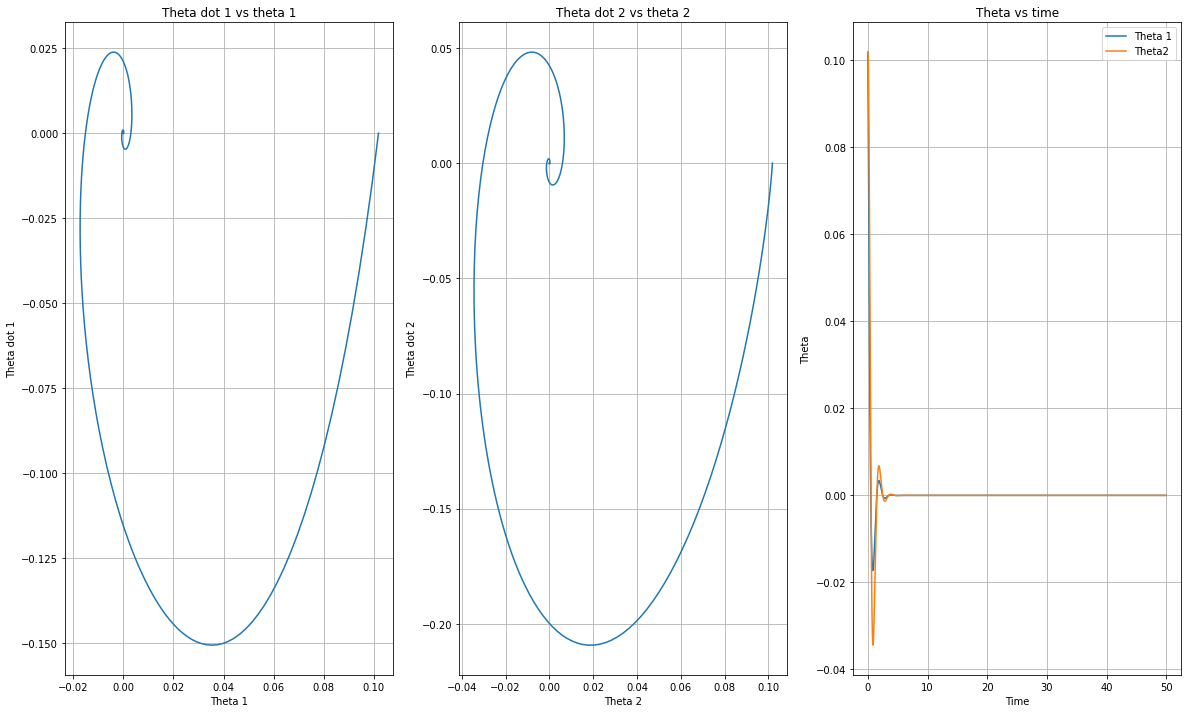
\includegraphics[scale=.30]{all.png}
    \caption{Graphs of the pendulums motion with initial conditions}
    \label{fig:code}
\end{figure}
The motion gets more complicated as the parameters are varied.
By making L1 longer than L2, the motion stays in a harmonic fashion but takes longer for the pendulums to return to the origin. Making L2 longer than L1, however, causes the phase space of the first pendulum to vary slightly as shown in the first graph in Figure 2. The first pendulum still follows a harmonic motion albeit with a slight deviation. This could be due to the first pendulum experiencing a jerk from the second pendulum.
\begin{figure}[H]
    \centering
    \centering
    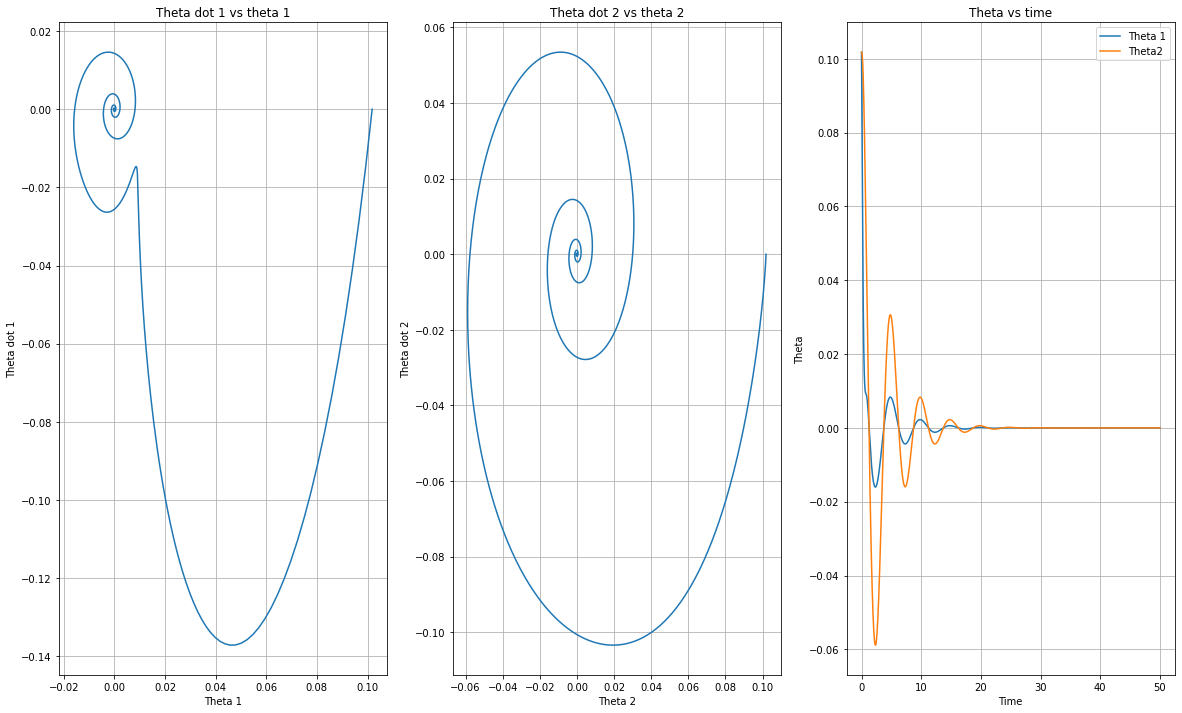
\includegraphics[scale=.30]{l2.png}
    \caption{Graphs of the pendulums motion with $L_2$ being longer}
    \label{fig:code}
\end{figure}
Manipulating the mass of the two pendulums produces interesting results. The increase of $m_1$ follows a similar general harmonic motion when comparing the first graphs in Figure 1 and 3 showing that $m_1$ is not as affected by the motion of $m_2$. The second and third graph in Figures 2 and 3 are similar except in Figure 2, the third graph takes longer for $\theta$ to settle to 0 showing that both pendulums experience much more movement.
\begin{figure}[H]
    \centering
    \centering
    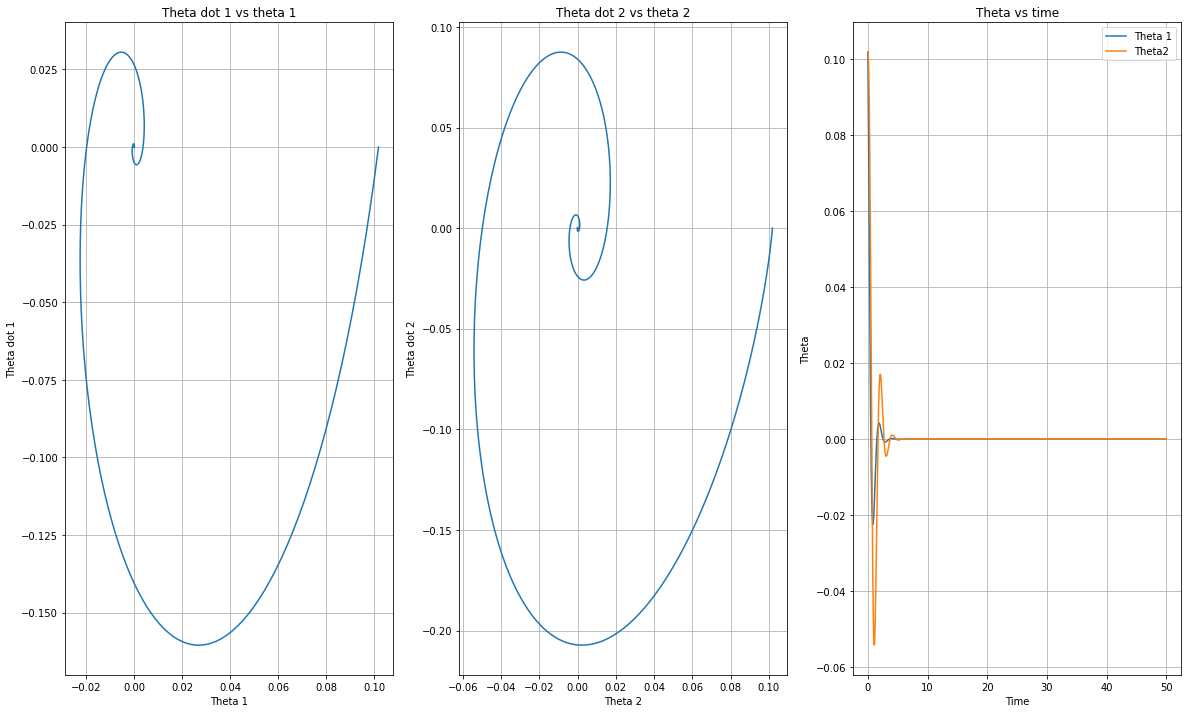
\includegraphics[scale=.30]{m1.png}
    \caption{Graphs of the pendulums motion with $m_1$ being larger than $m_2$}
    \label{fig:code}
\end{figure}
On the contrary, making $m_2$ to be larger than $m_1$ causes the movements of both pendulums to become much more stiff and come to rest much more quickly as demonstrated by Figure 4. In graphs 1 and 2 of Figure 4, the velocity decreases and $\theta$ reduces sharply before coming to rest, further shown by their relative positions in graph 3.
\begin{figure}[H]
    \centering
    \centering
    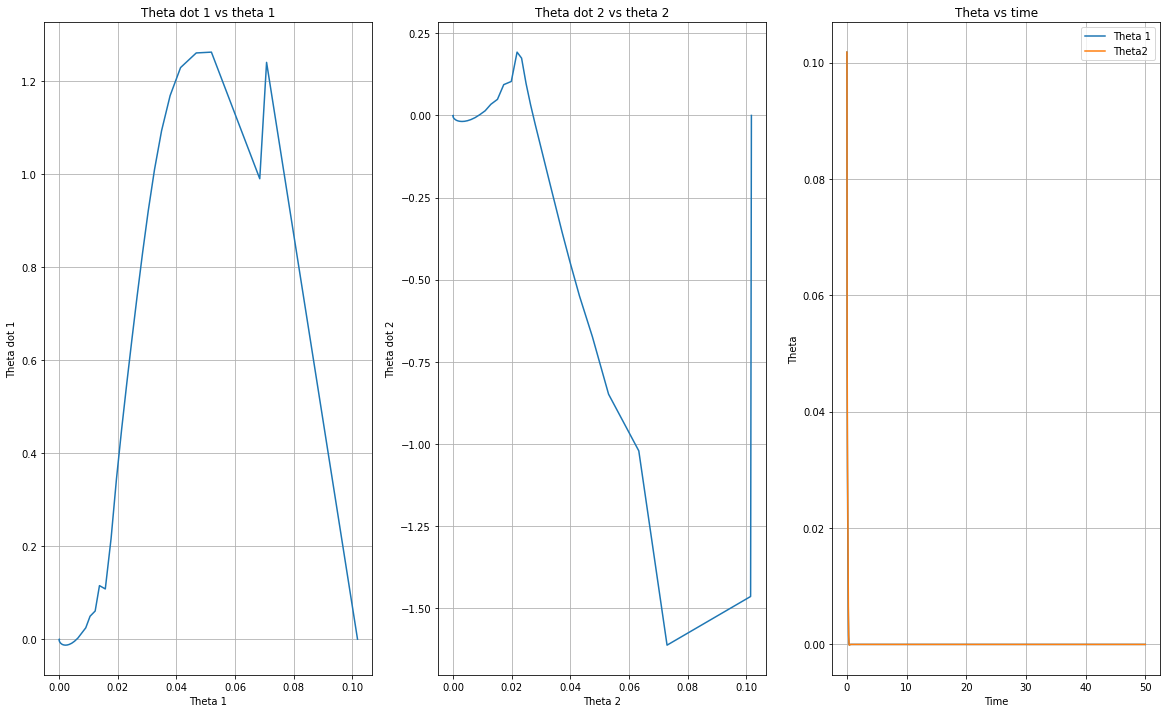
\includegraphics[scale=.30]{m2.png}
    \caption{Graphs of the pendulums motion with $m_2$ being larger than $m_1$}
    \label{fig:code}
\end{figure}
Depending on the pendulums' positions, their movements can be described as irregular. As shown in Figure 5, adjusting the angle of the first pendulum causes the first and second pendulum to follow a slightly modified form of a harmonic motion. Adjusting the second pendulum to be have a greater angle than the first pendulum reverses the positions as shown by Figure 6 albeit with more motion. 
\begin{figure}[H]
    \centering
    \centering
    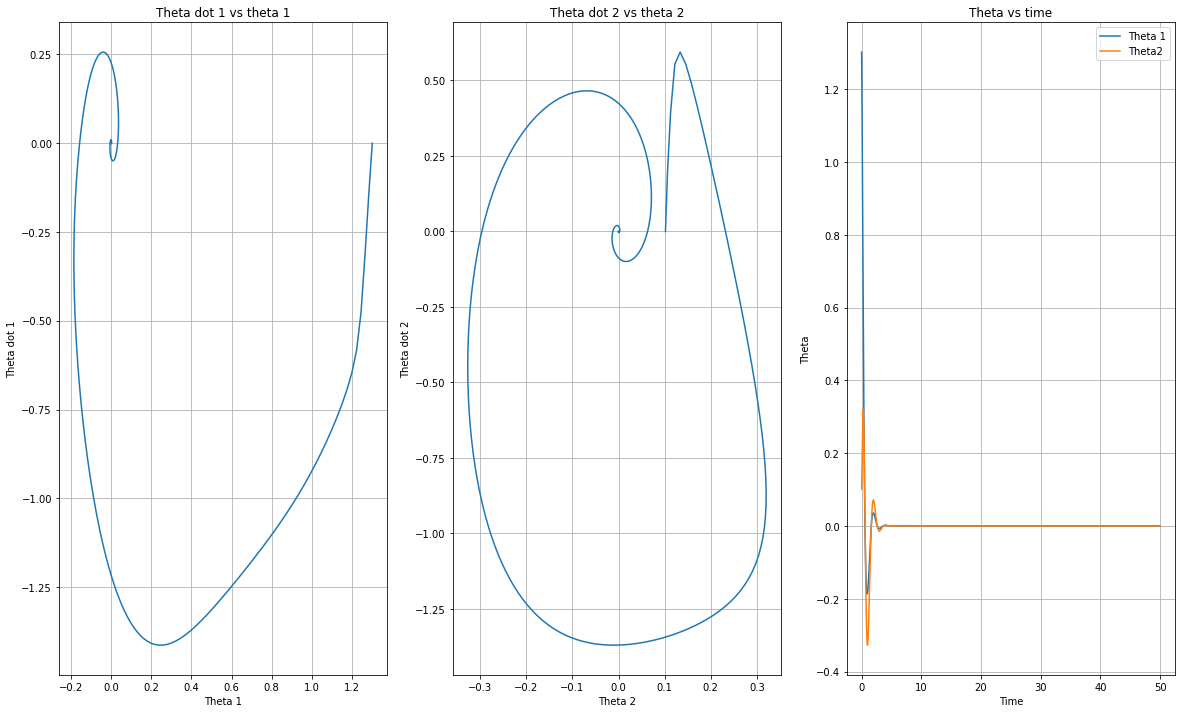
\includegraphics[scale=.30]{theta1.png}
    \caption{Graphs of the pendulums motion with $\theta_1$ being increased}
    \label{fig:code}
\end{figure}
\begin{figure}[H]
    \centering
    \centering
    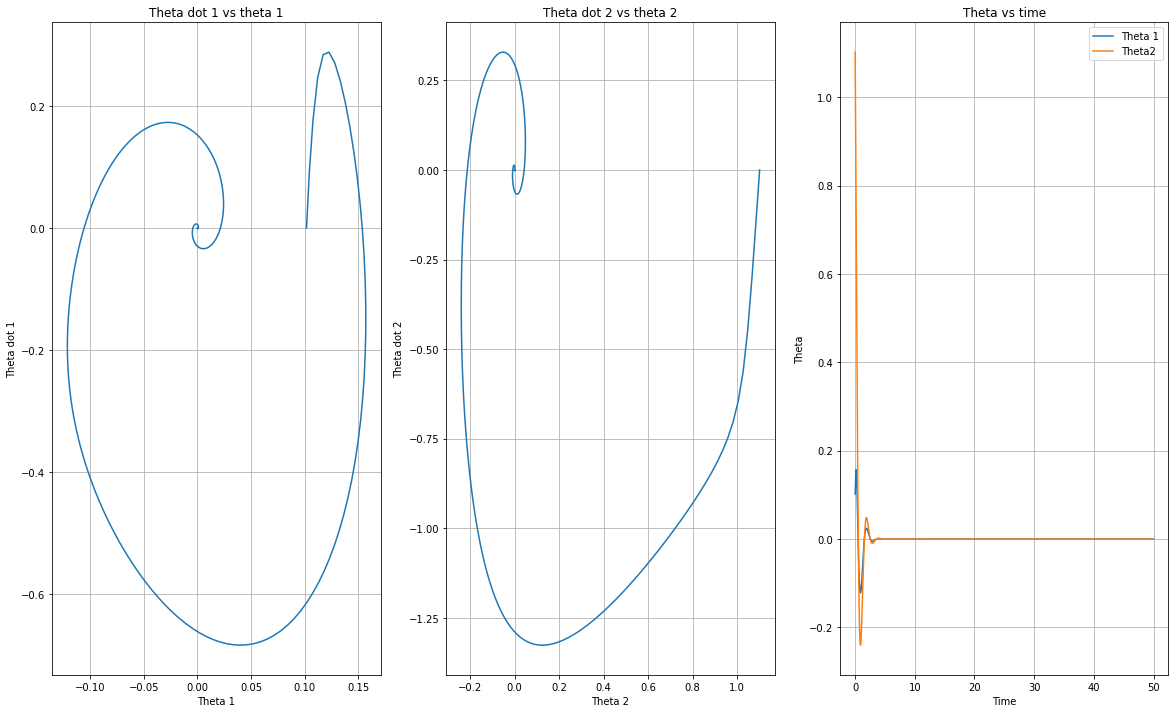
\includegraphics[scale=.30]{theta2.png}
    \caption{Graphs of the pendulums motion with $\theta_2$ being larger than $m_1$}
    \label{fig:code}
\end{figure}
With the addition of an initial velocity to either pendulum, the movements of both pendulums follow a simple harmonic path up until a certain point, approximately 4.7 for $\dot\theta_1$ and 5 for $\dot\theta_2$. As demonstrated by both figures 7 and 8, at least one pendulum spikes to a large angle with varying velocities before coming to a standstill. Adjusting the velocities to the aforementioned results in at least one pendulum not coming to a standstill as show in Figures 9 and 10.
\begin{figure}[H]
    \centering
    \centering
    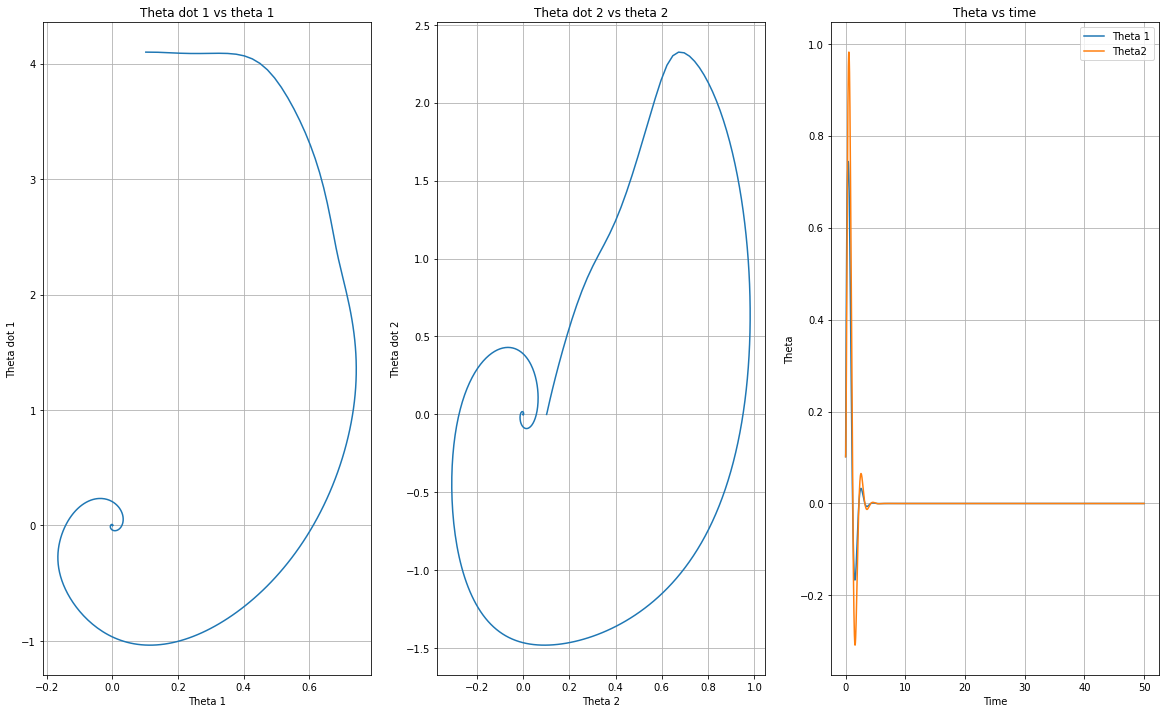
\includegraphics[scale=.30]{td1.png}
    \caption{Graphs of the pendulums motion with $\dot\theta_1$ being increased}
    \label{fig:code}
\end{figure}
\begin{figure}[H]
    \centering
    \centering
    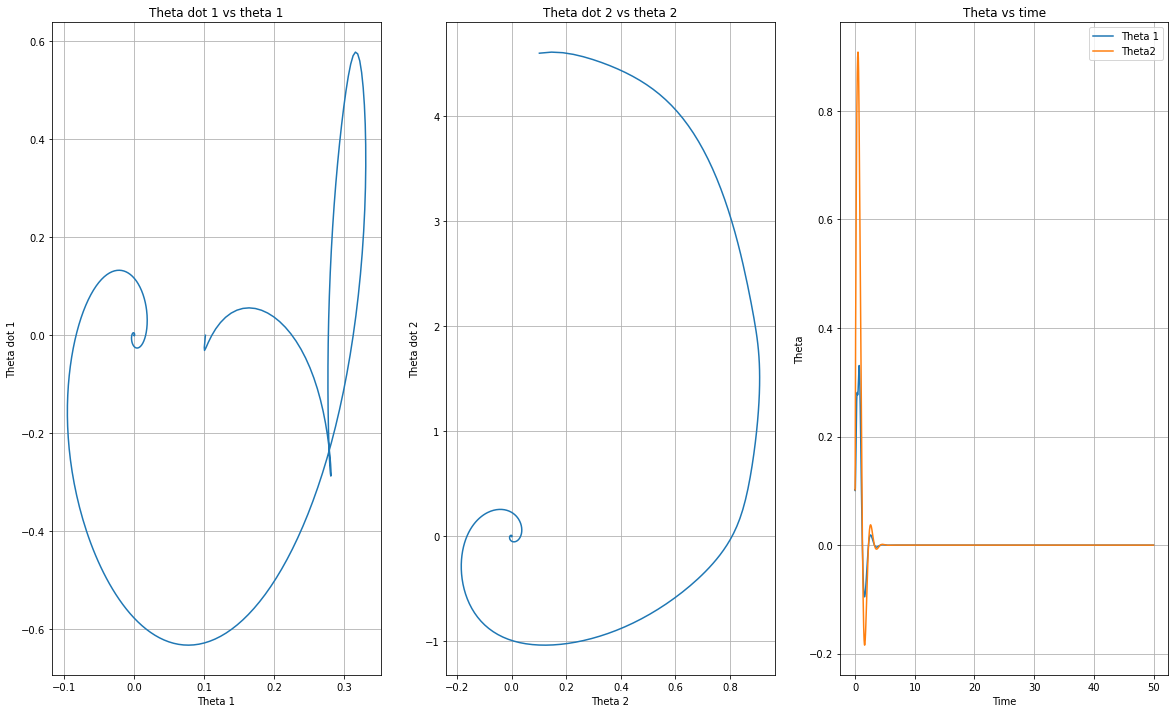
\includegraphics[scale=.30]{td2.png}
    \caption{Graphs of the pendulums motion with $\dot\theta_2$ being increased}
    \label{fig:code}
\end{figure}
\begin{figure}[H]
    \centering
    \centering
    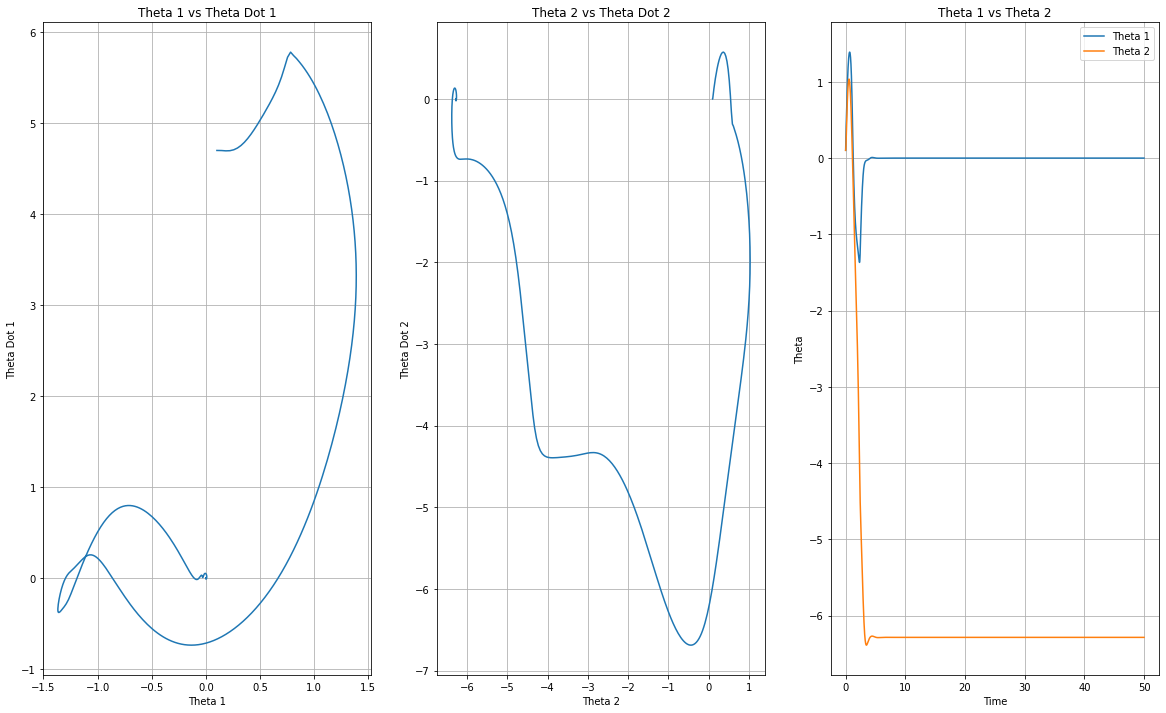
\includegraphics[scale=.30]{thetadot1.png}
    \caption{Graphs of the pendulums motion with $\dot\theta_1$ at 4.6}
    \label{fig:code}
\end{figure}
\begin{figure}[H]
    \centering
    \centering
    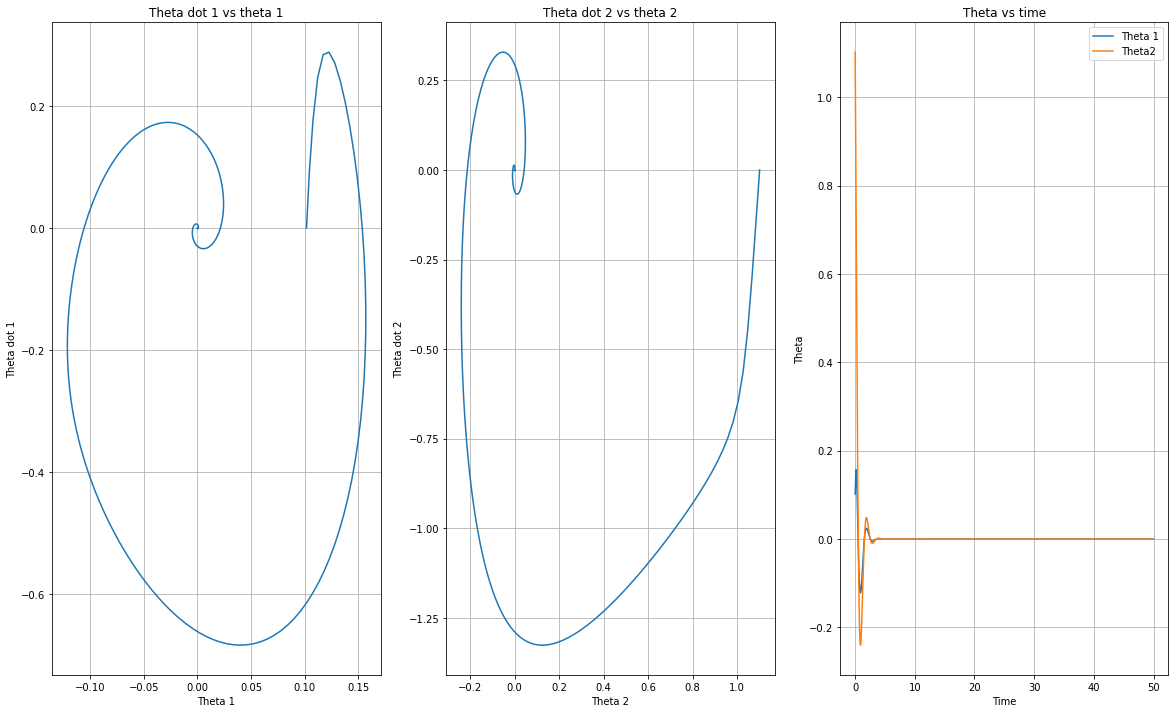
\includegraphics[scale=.30]{theta2.png}
    \caption{Graphs of the pendulums motion with $\dot\theta_2$ at 5.00}
    \label{fig:code}
\end{figure}
So far, the discussion has primarily been over manipulating one parameter while keeping all other parameters the same as the initial conditions. Combining different parameters produces different motions that can be described as chaotic. A manipulation of the parameters involving the lengths of the strings or the masses produces movements that remain harmonic or akin to it. One such example is adjusting $L_1$ and $m_1$ to be larger than their counterparts as shown in Figure 11. Here, the pendulums swing in a back and forth manner before coming to a standstill. 
\begin{figure}[H]
    \centering
    \centering
    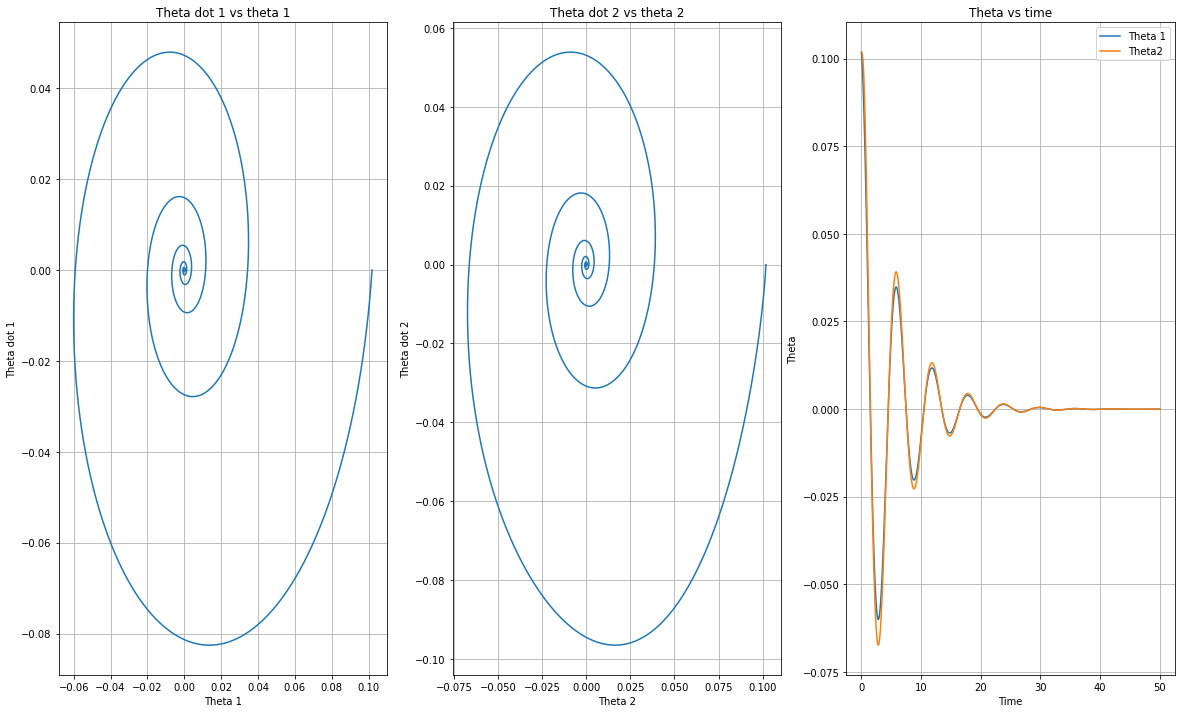
\includegraphics[scale=.30]{l1m1.png}
    \caption{Graphs of the pendulums motion with $L_1$ and $m_1$ being increased}
    \label{fig:code}
\end{figure}
\begin{figure}[H]
    \centering
    \centering
    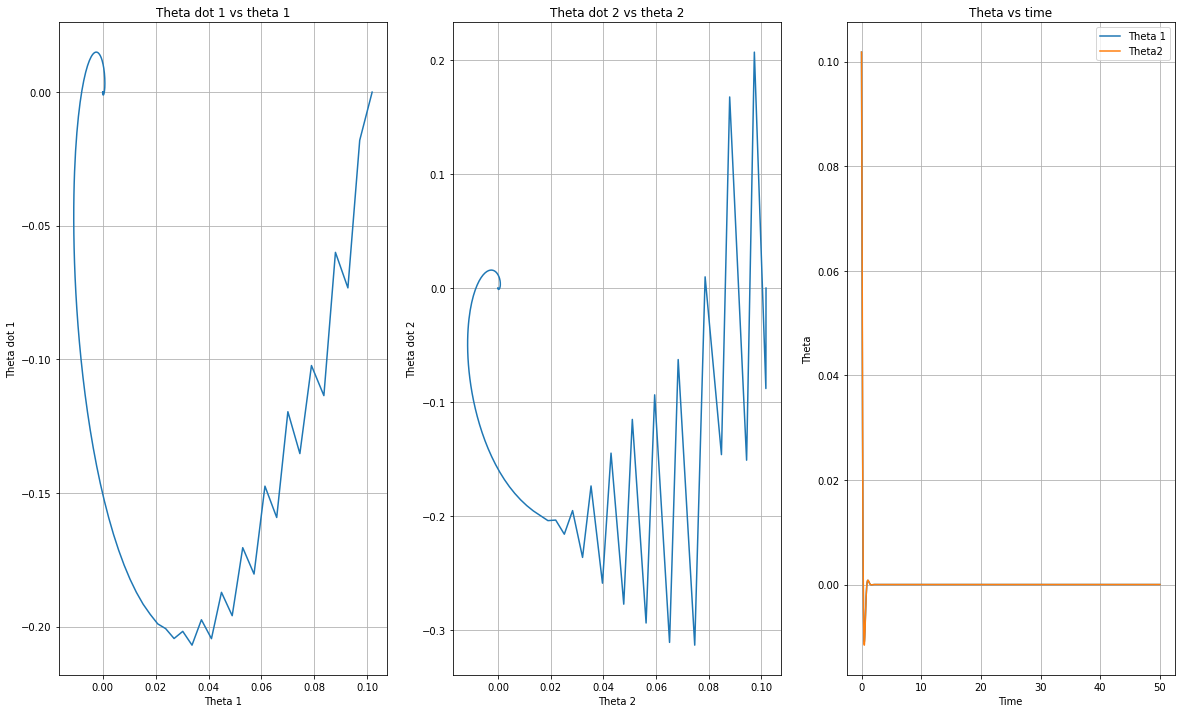
\includegraphics[scale=.30]{l1m2.png}
    \caption{Graphs of the pendulums motion with $L_1$ and $m_2$ being increased}
    \label{fig:code}
\end{figure}
However, the introduction of the initial angles and initial velocities causes the pendulums to follow a non-harmonic path. As shown in Figure 12, the first pendulum eventually comes to rest but the second pendulum continues moving past the time allotted for the experiment. Analyzing the first two graphs show chaotic movement among the pendulums. The first pendulum follows a quivery path while the second pendulum continues to increase its velocity along with its angle. 
\begin{figure}[H]
    \centering
    \centering
    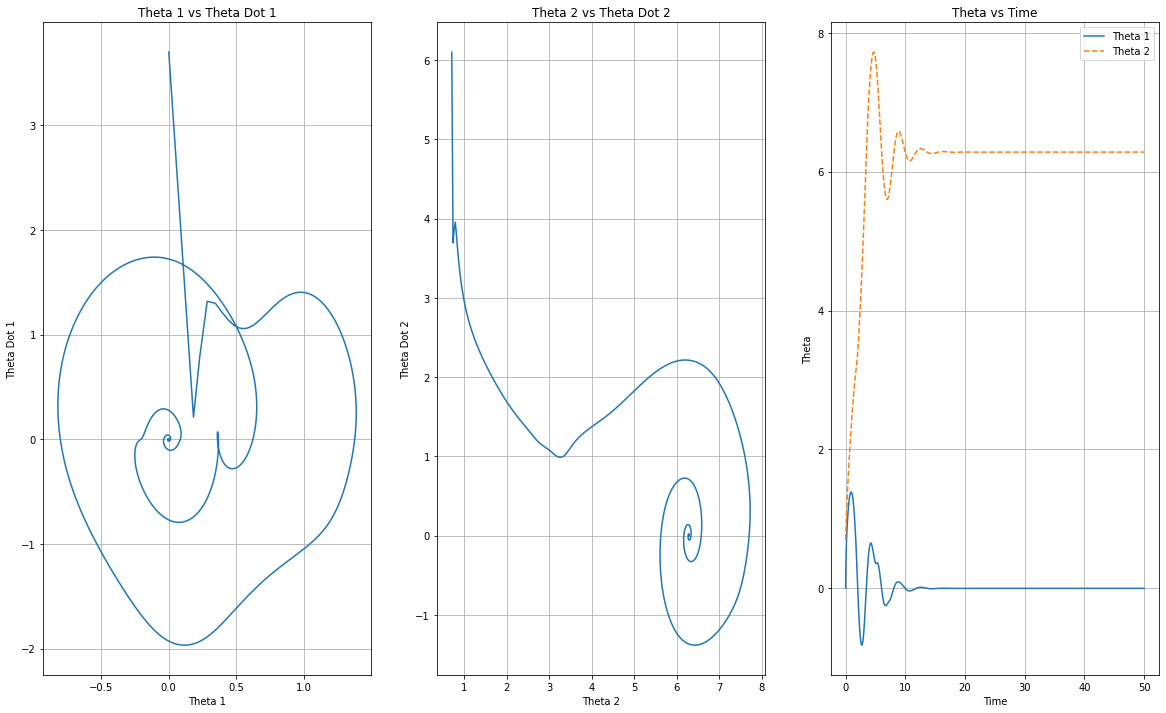
\includegraphics[scale=.30]{wonky.png}
    \caption{Graphs of the pendulums motion with $L_2$, $m_2$, $\theta_1$, $\theta_2$, $\dot\theta_1$, and $\dot\theta_2$ being increased}
    \label{fig:code}
\end{figure}
There are many different types of combinations parameters that can be created, producing interesting movements but will not be explored for consideration of the paper's length. Further animation can be found through the link: \href{https://drive.google.com/file/d/10Jvuc9amuOyc7-DA5pSDOUm4YVg-A3B9/view?usp=share_link}{Animation}
\href{https://colab.research.google.com/drive/13S_AaAXCl-azm20LnW0CQ7vJEFCP3yjH?usp=sharing}{Interactive Plots}
\section{Conclusion} \label{sec:conclusion}
Through these investigations, the results show that a seemingly simple double pendulum can display complex behavior. The seemingly deterministic system is actually unpredictable. The double pendulum displays quasi-harmonic motion when the deviation from equilibrium is small (see figure 1). Intriguing patterns emerge as larger deviations from equilibrium were investigated (see figures 2-13). These plots show that the differential equations used to model the motions of the double pendulum display non-linearity, disrupting the deterministic nature of the double pendulum system and rather creating chaos. Although there are a set of equations defining this system, it is still intrinsically unpredictable due to unavoidable errors encountered physically and/or numerically. 

There are several ways the double pendulum system can still be explored. Firstly, the equations were derived assuming that there was no friction, air resistance, or noise introduced to the system. Adding these forces could can make the system more unpredictable by adding to the non-linearity of the equations. Additionally, with these forces added the chaos would eventually slow down as it will cause energy will dissipate from the pendulum, eventually leading to the pendulums halting. Future work could be aimed at adding the drag force into the derivation of motion to make the system more pragmatic and investigating how this force affects chaos by either using the numerical method discussed in this paper or ODE solvers. Secondly, we assumed that both pendulums were restricted to the same plane; however, if one pendulum was oscillating on the x-z plane and the other pendulum was oscillating on the y-z plane, this would completely change the direction of the derivations of motion. Exploration on modeling the motion for a system with two planes could reveal further information about the chaotic nature of the double pendulum system that could have further real life applications based on the dynamics of the system.   


\newpage
\bibliographystyle{ieeetr}
\bibliography{citation.bib}

\section{Acknowledgements} \label{sec:acknowledgements}
We would like to express our gratitude to Brett Barkley and Dr. Shaymal Mitra for their guidance and lectures. 

\end{document}

